% lualatex statestikz-2.tex
% or
% then
% pdf2svg statestikz-2.pdf statestikz-2.svg

\documentclass[border=2bp, tikz]{standalone}
\usepackage{tikz}

\usetikzlibrary{calc,trees,matrix,positioning,chains,fit,intersections}
\usetikzlibrary{arrows,shapes.arrows,shapes.geometric,shapes.multipart,shapes.symbols}
\tikzset{
   state/.style={ rectangle, draw=black, thick, minimum height=1.66em, text centered, rounded corners=3pt},
   error state/.style={ rectangle, double, draw=black, semithick, minimum height=1.66em, text centered, rounded corners=3pt},
   off state/.style={ circle, double, draw=black, semithick, minimum height=1.66em, text centered, rounded corners=3pt},
   branch/.style={ fill, shape=circle, minimum size=3pt, inner sep=0pt},
   cross line/.style={preaction={draw=white, -, shorten >=2pt, shorten <=2pt, line width=2.5pt}},
   >=latex
}
\usepackage{fontspec}
\setmainfont[UprightFont={Petrona-Light.ttf},
             BoldFont={Petrona-Semibold.ttf},
             ItalicFont={Petrona-LightItalic.ttf},
             BoldItalicFont={Petrona-SemiBoldItalic.ttf},
            ]{Petrona-Light.ttf}

\begin{document}
\begingroup
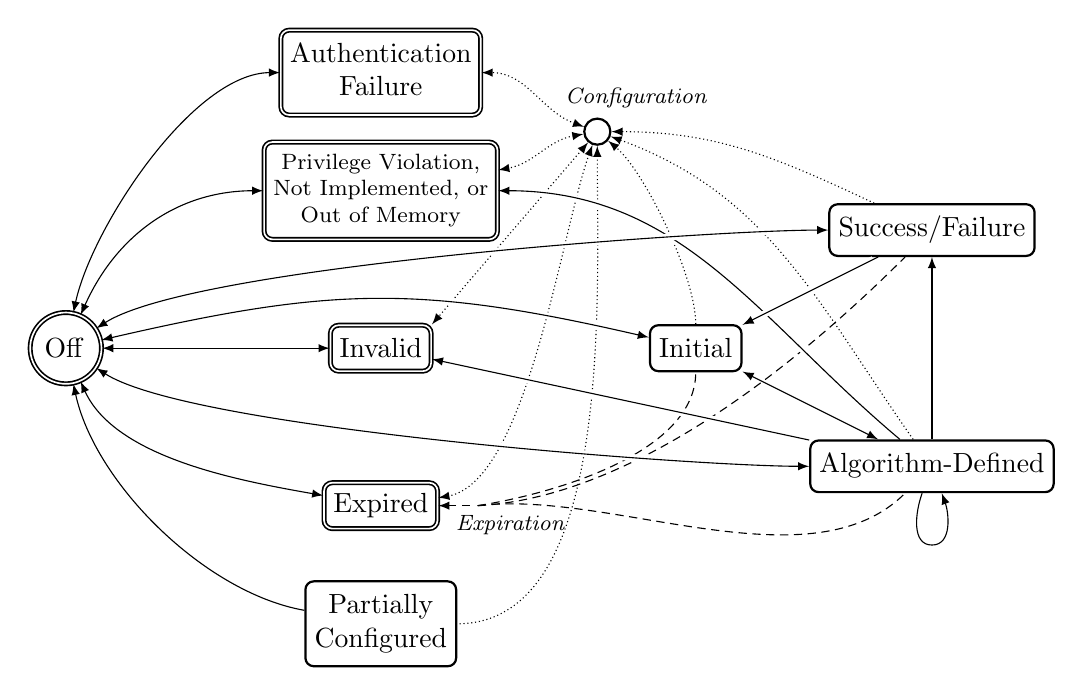
\begin{tikzpicture}
  \node[off state]  at (-2,0)    (off)            {Off\,};

  \node[error state] at (2,0)    (invalid)        {Invalid};
  \node[error state] at (2,2)    (various errors) {\footnotesize\begin{tabular}{@{}c@{}}Privilege Violation,\\Not Implemented, or\\Out of Memory\end{tabular}};
  \node[error state] at (2,3.5)  (authfail)       {\begin{tabular}{@{}c@{}}Authentication\\Failure\end{tabular}};
  \node[error state] at (2,-2)   (expired)        {Expired};
  \node[state]       at (2,-3.5) (partial)        {\begin{tabular}{@{}c@{}}Partially\\Configured\end{tabular}};

  \node[circle,thick,draw=black] at (4.75,2.75) (configuration hub) {};
  \node[above=0mm  of configuration hub,xshift=5mm] (ignore) {\footnotesize \textit{Configuration}};

  \node[coordinate] at ($(expired.east)+(0.5,0)$) (before expired) {};
  \node[below right=0mm and -4mm of before expired] (ignore) {\footnotesize \textit{Expiration}};

  \node[state, thick] at (6,0)  (initial)           {Initial};
  \node[state, thick] at (9,-1.5) (algorithm defined) {\begin{tabular}{@{}c@{}}Algorithm-Defined\end{tabular}};
  \node[state, thick] at (9,1.5)  (success failure)   {\begin{tabular}{@{}c@{}}Success/Failure\end{tabular}};

  \draw[->,densely dotted]  (initial)            to[out=90,in=-40,looseness=0.6] (configuration hub);
  \draw[->,densely dotted]  (algorithm defined)  to[out=125,in=-20] (configuration hub);
  \draw[->,densely dotted]  (success failure)    to[out=155,in=0] (configuration hub);
  \draw[<-,densely dotted]  (configuration hub)  to[out=270,in=0,looseness=0.8] (partial);
  \draw[<->,densely dotted] (configuration hub)  to[out=160,in=0] (authfail);
  \draw[<->,densely dotted] (configuration hub)  to[out=190,in=10] (various errors);
  \draw[<->,densely dotted] (configuration hub)  -- (invalid.north east);
  \draw[<->,densely dotted] (configuration hub)  to[out=250,in=10,looseness=0.6] ($(expired.east)+(0,0.1)$);

  \draw[-,densely dashed]  (before expired) to[out=9,in=270,looseness=0.8] (initial);
  \draw[-,densely dashed]  (before expired) to[out=7,in=225,looseness=0.8] (algorithm defined);
  \draw[-,densely dashed]  (before expired) to[out=3,in=225,looseness=0.8] (success failure);
  \draw[->,densely dashed] ($(before expired)+(-0.1,0)$) -- (expired);

  \draw[<->] (off) -- (invalid);
  \draw[<-]  (off) to[out=282,in=170,looseness=0.8] (partial);
  \draw[<->] (off) to[out=78,in=180,looseness=0.7] (authfail);
  \draw[<->] (off) to[out=66,in=180] (various errors);
  \draw[<->] (off) to[out=294,in=170,looseness=0.8] (expired);

  \draw[<->] (initial) -- (algorithm defined);

  \draw[->,cross line] (algorithm defined) -- (success failure);

  \draw[->] (algorithm defined) to[out=250,in=180] ($(algorithm defined)+(0,-1)$) to[out=0,in=290] (algorithm defined);
  \draw[->, cross line] (algorithm defined) -- (invalid);
  \draw[->,cross line] (algorithm defined) to[out=140,in=0] (various errors);

  \draw[<->,cross line] (off) to[out=13,in=167,looseness=1.1] (initial);
  \draw[<->,cross line] (off) to[out=-33,in=180,looseness=0.4] (algorithm defined);
  \draw[->,cross line] (success failure) -- (initial);
  \draw[<->,cross line] (off) to[out=33,in=180,looseness=0.4] (success failure);

\end{tikzpicture}
\endgroup
\end{document}
